\chapter{Experimental Design}
\label{Ch2}

In the bouncing droplet system we observe a unique interaction between a droplet and it's wave that showcases various novel behaviours under different circumstances.  In the experiments discussed herein, we will look at how features \textit{underneath} the surface of the oil (i.e. on the ``floor" of the tray) affect the motion of the droplet. 

A raised object on the floor of the tray (but still underneath the surface of the oil) can have an effect on height of the surface waves, and thus, on the motion of the walker\rf{tunneling}. Sometimes a droplet headed towards a raised object will be reflected backwards, as if from a collision with the object. For this reason, we refer to a raised object as a barrier, because it impedes the motion of the droplet. Oftentimes however, the droplet slows down, but continues on and crosses the barrier without a collision. This is analagous to ``transmission" in the quantum mechanical process of tunneling. For a given barrier of a certain height and width, we will see a probability of tunneling unique to that barrier. Other studies have shown that increasing barrier width decreases probability of tunneling\rf{tunneling}. This study looks at how height of the barrier affects the tunneling probability. 

To test the effect of a barrier's height on the probability of tunneling, I used a combination of procedures from the investigations of Bush\rf{pilot-wave}, Couder\rf{Couder2005a}, and specifically, Eddi et al.\rf{tunneling}. These were slightly modified to fit some of the unique features of my experiment. In this section, I aim to give some of the reasoning behind the  design of the experimental apparatus and data collection techniques, both of which are not well described in the literature.

\section{Setup}
    The schematic of the experimental setup is shown in \refFig{setup}, and a picture of the actual setup is shown in \refFig{group}(a). A waveform generator creates a sinusoidal signal which is amplified and fed into a shaker. This signal drives shaker, which vibrates the tray vertically. Both the frequency and the amplitude of the vertical oscillations can be controlled. An accelerometer records the vertical acceleration of the tray and is read by an oscilloscope. A camera records the droplet as it bounces along the surface of the oil.  
    
   
    
\begin{figure}[h!]
	\centering
	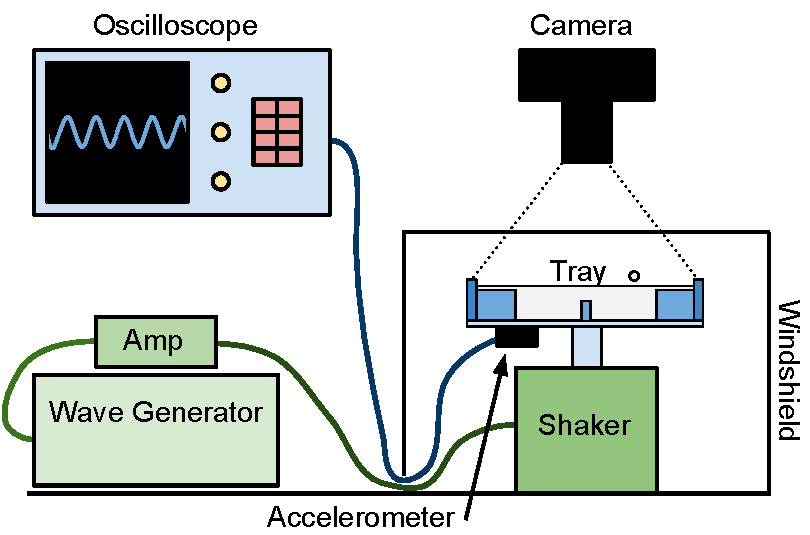
\includegraphics[scale=0.8]{Setup.pdf}
	\caption{The experimental setup. The amplified signal from the wave generator drives the shaker, which shakes the oil-filled tray. The accelerometer generates a signal which is read by the oscilloscope. The shield blocks disturbances to the experiment, while allowing the camera to document the trials.}
	\label{setup}
\end{figure}

\section{Materials}
The key components of this experiment are the shaker, the oil, and the tray. In this section I will describe the specifics of this holy trinity, as well as some of the additional components used in data collection. 

\subsection{Tray}
The tray was fabricated from acrylic plastic parts that were cut on the Trotek Rayjet 300 laser cutter. The manufactured components were then glued together with Scigrip Weld-On 3 assembly adhesive. The tray's design, which was based off of the tray in the tunneling experiment done by Eddi et al.\rf{tunneling}, naturally guides the droplet into a perpendicular collision with the barrier. The tray schematic is shown in \refFig{tray}. 

\begin{figure}[h!]
	\centering
	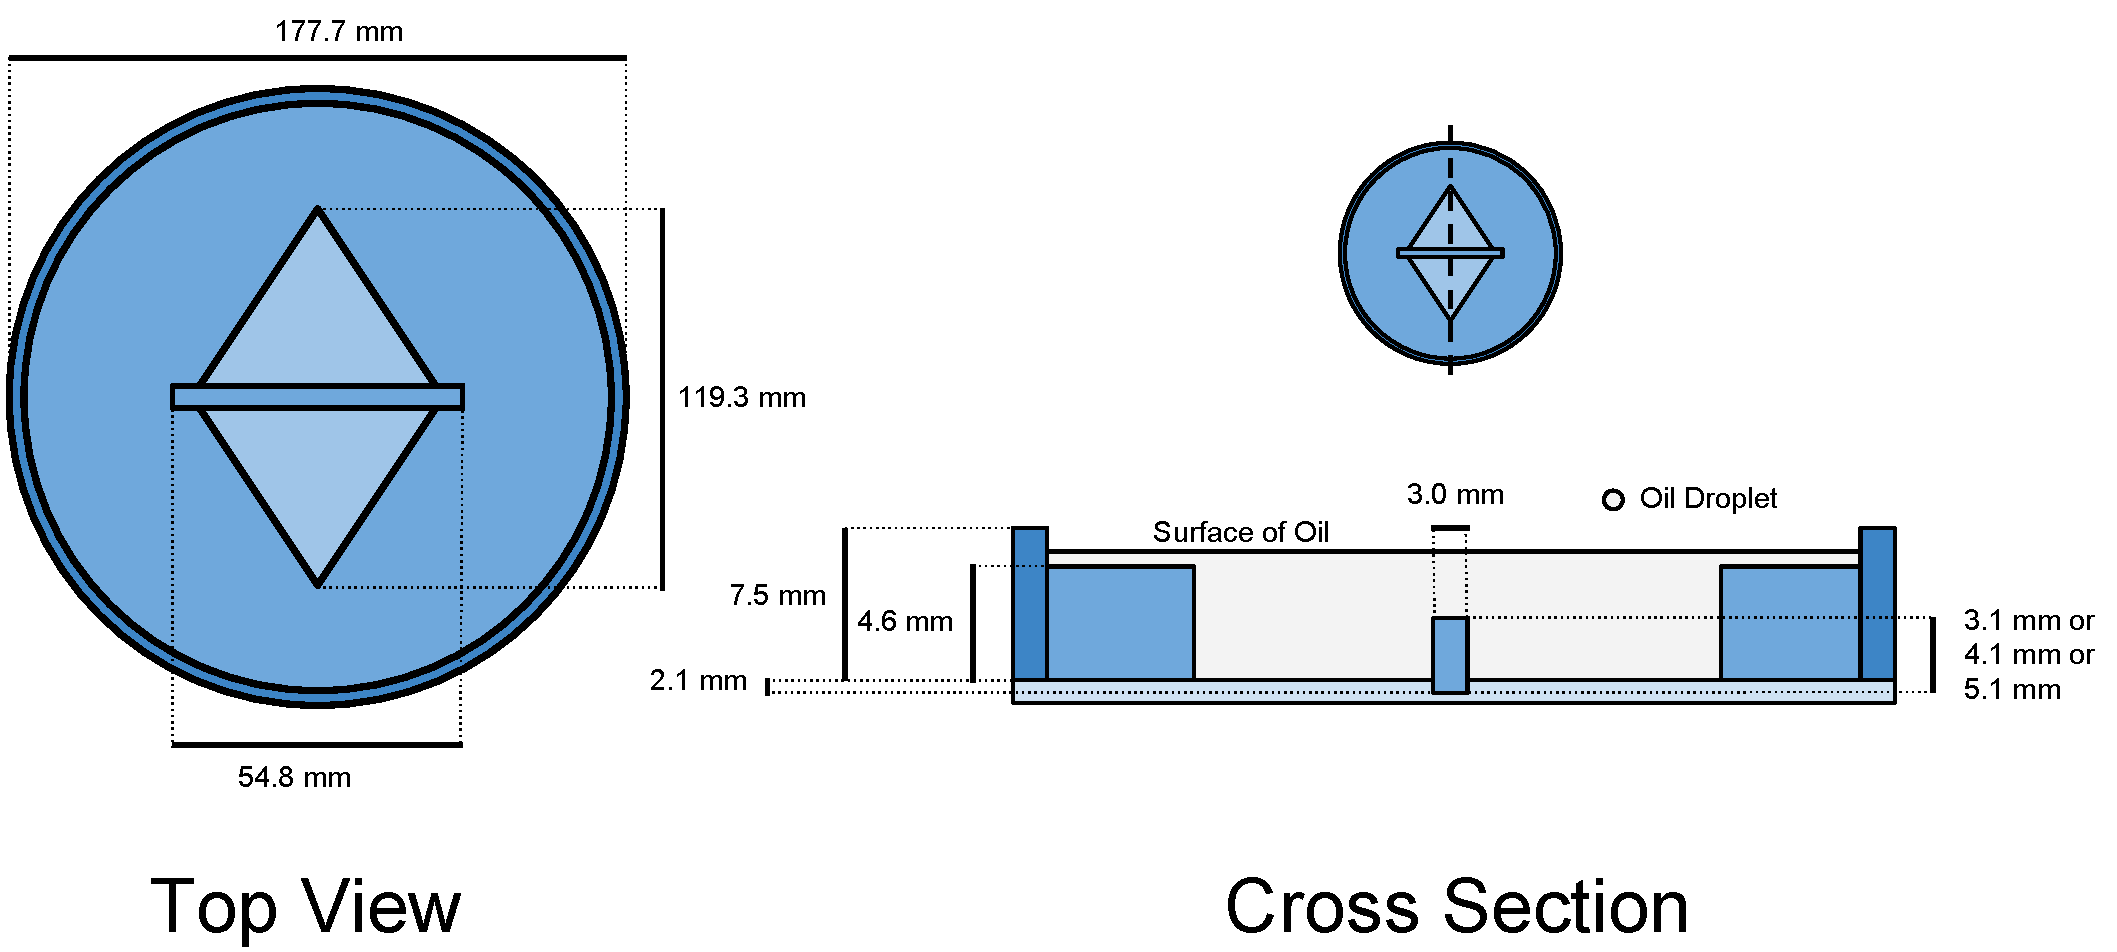
\includegraphics[scale=0.48]{Tray.pdf}
	\caption{The specifications of the tray design. The top view (left) highlights the main elements in the tray, while the cross section (right) illustrates the topography of the tray. Depth is represented by the shading; darker shading is shallower.}
	\label{tray}
\end{figure}

A thin layer of oil spills over the constraining rhombus shape. As long as the layer is thin enough, the droplet will remain in the rhombus container, but the waves will continue to propagate unimpeded. This gives the waves time to decay, and means that the droplets motion is not affected by reflections of previous waves from the sidewalls, and is instead guided only by the unreflected waves. 

The rhombus shape serves to steer the droplet into a perpendicular collision with the barrier. This forces the droplet to pin-ball into the acute corner of the rhombus and shoot out towards the barrier as shown in \refFig{group}(c).

I designed my experiment to test barriers of three different heights: $2.75~\mathrm{mm}$, $3.0~\mathrm{mm}$, and $3.25~\mathrm{mm}$, measured from the bottom of the rhombus. A thin barrier of plastic made by the laser cutter has the tendency to bend and warp over time. To avoid this problem, we made the barriers taller than the specified heights. Then we created a cut-out in the rhombus so the barriers could be inserted and held in place by the tight fit. The barrier cut-outs were deep enough to exactly counter the added height of the barrier, so the barriers still had (when measured from the surface of the rhombus) heights of $2.75~\mathrm{mm}$, $3.0~\mathrm{mm}$, and $3.25~\mathrm{mm}$. This also solved the problem of fixing the barriers in place, while still allowing them to be easily removed. The particular heights of the barriers were chosen because they allowed for both passage over and blockage by the barriers depending on the parameters. Other barriers that were too tall blocked all of the droplets, while barriers that were too short did nothing to prevent the droplet from crossing over.

The bottom of the tray was painted black in order to improve contrast, allowing the droplet to be more easily tracked by eye and using a camera.

\begin{figure}[h!]
	\centering
	\includegraphics[scale=0.55]{group.pdf}
	\caption{(a)~The actual experimental setup. 
	(b)~The screen of the oscilloscope, showing the output from the accelerometer. The sine wave is the acceleration of the tray, and records a frequency $79.9954~\mathrm{Hz}$ and a peak to peak voltage of $158~\mathrm{mV}$. 
	(c)~The path of a droplet of width $0.87~\mathrm{mm}$, highlighted in red, shows the droplet's motion as it walks into a corner before shooting out directly towards the barrier (orange).}
	\label{group}
\end{figure}

\subsection{Silicone Oil}
    Silicone oil was the ideal choice of fluid for this experiment because it remains clean, it has a low vapor pressure (so it does not evaporate), and it can be purchased at specific viscosities. The silicone oil used in this experiment had a viscosity of 20 cSt (its viscosity is a little closer to water than olive oil) and was purchased from Clearco Products Co. Inc., Bensalem PA (CAS No: 63148-62-9). 20 cSt silicone oil, like the one used by Bush et al.\rf{pilot-wave} was chosen because it exhibits walking behaviour under a wider range of parameters\rf{pilot-wave} than more viscous oil, such as the 50 cSt viscosity oil used by Couder\rf{Couder2005a}. Depending on the height of the barrier and the desired height of oil above the barrier, the tray requires around $18.0~\mathrm{mL}$ of fluid. This volume of oil left a different depth of oil above the barrier, depending on which barrier was in place. For the shortest barrier of $2.75~\mathrm{mm}$, the depth of the oil on top of the barrier was $1.5~\mathrm{mm}$. The middle barrier of height $3.0~\mathrm{mm}$ had about $1.25~\mathrm{mm}$ of fluid above it. The tallest barrier at $3.25~\mathrm{mm}$, only had $1.0~\mathrm{mm}$ of fluid on top.
    
    It was of vital importance to keep the oil as clean as possible since any surface contamination leads to droplet coalescence. This meant protecting the oil from particulate matter that was already in the tray. Contamination was minimized by cleaning the tray before filling it and shielding it from the ambient dust.
    
\subsection{Shaker}
    To shake the tray, we used a mechanical wave driver made by Pasco Scientific, Roseville CA, model SF-9324. An acrylic component was attached to the bottom of the tray, so that the tray was fastened to the thin rod that came from the shaker. This juncture was tightened with a screw.
    
    This shaker was designed to drive a string or an elastic cord, not a $200~\mathrm{gram}$ tray with oil inside. In other words, the shaker was probably at the limit of what it was designed to handle. As a result, there was notable decrease in performance after just a couple of minutes of vibration. The initial behavior could be partially recovered after an hour long rest, but after weeks of use there was a noticable difference. This difference was mainly the in acceleration; towards the end of a trial, a signal with a higher amplitude had to be generated to produce the same accelerations as from the beginning of the trial. For this reason, the shaker was replaced right before collecting the raw data and was allowed a resting period before begining the following trial. The damping of the vibrations also meant that the acceleration signals from the accelerometer had to be continuosly  monitored, since the constant signal from the wave generator could not be trusted to produce a constant tray vibration. 
    
\subsection{Waveform Generator and Amplifier}
    The shaker was driven with an Agilent Arbitrary Waveform Generator model 33210. This was controlled digitally and was found to be more stable than other available frequency generators. The waveform generator was usually set to produce a sine wave of $80~\mathrm{Hz}$. The signal from the waveform generator was amplified using a Lepai LP2020A+ digital amplifier. This precise control of the the amplitude of the tray. This signal, which was also measured with a multimeter, was then fed into the shaker.    
            
\subsection{Accelerometer}  
    As discussed in \refChapter{Ch1}, knowing the tray's acceleration allows us to characterize the behavior of our system. To measure acceleration, we attached an ADXL 326 triple axis accelerometer (made by Adafruit, New York City NY) to the bottom of the tray. Using screws, provided a much firmer hold than tape or glue while allowing for removal. The ADXL 326 has a range of $\pm$16$g$, which is ideal for measuring the accelerations in our setup, usually below $5g$'s. 
      
      The signal from the z-axis of the accelerometer was measured directly on a Tektronix TDS 2012C oscilloscope, a sample output can be seen in \refFig{group}(b). For the vibrating tray, the output was approximately sinusoidal (as expected). The spec sheet for the accelerometer indicates that the sensitivity can be translated to $57 \pm 6~\mathrm{mV/g}$. 
    
\subsection{Shield}
    A large, see-through cylinder (covered at one end) was manufactured using the laser cutter. When placed over the tray, it served the purpose of keeping the oil clean from particulate matter and preventing air currents from influencing the motion of the walker.       
   
\subsection{Leveling Platform}
    A wooden leveling platform supported the shaker. Three adjustment screws allowed for precise adjustment of the tilt of the apparatus. The tray was tuned using a level placed inside the center of the tray (before the oil was added). 

\subsection{Camera}       
 
To document trials we used a Canon EOS Rebel T5i DSLR camera supported on a tripod and aimed directly down at the tray. Attached to the camera was a Canon 18-135 mm lens. Set with a Tv configuration (Time Value -- allows for shutter control) and in video mode, the 18 MP image could be optically zoomed and manually focused on the bouncing droplet. 

\section{Procedure}
Once the exact walking parameters were established (frequency and driving amplitude), tunneling measurements at a few different barrier heights were made. 

\subsection{Finding the Walking Regime}

Before investigating the rate of tunneling using different barriers, a rough estimate of the walking regime at a frequency of $80~\mathrm{Hz}$ must be made. A ``map" detailing the walking and bouncing threshold for different frequencies and amplitudes was produced. Reproducing this figure allows us to find the parameters that are specific to our unique setup, which could have slightly different height, tray, oil, and shaker configurations than those used in the literature. 

Droplet size is measured using a recorded video of the walking droplet in motion. By comparing the number of pixels making up the diameter of the droplet (unknown measurement) to the number of pixels making up the diameter of the tray (known measurement), we can estimate the length associated with  each pixel, and thus find the diameter of the droplet in millimeters. For accurate droplet diameter measurements, a mean value composed of 9 separate  droplet diameter measurements per trial trial was computed. The droplets had diameter on the order of $1.0~\mathrm{mm}$, as discussed in \refSect{parameters}. 

Driving acceleration values are measured by the accelerometer and displayed on the oscilloscope. To keep the acceleration constant across a measurement, the amplitude of the signal coming into the shaker was conitously increased in order to counteract the damping of the shaker.

To ensure that every trial has the same oil depth, we measured the volume of oil ($18.0~\mathrm{mL}$) before filling the tray using a $25~\mathrm{mL}$ graduated cylinder. Knowing the volume of the tray and of each barrier, we could calculate a value for the oil depth without interfering with the system. In this way, oil depth of oil above the barrier ($1.5~\mathrm{mm}$ for the $2.75~\mathrm{mm}$ barrier, $1.25~\mathrm{mm}$ for the $3.0~\mathrm{mm}$ barrier, $1.0~\mathrm{mm}$ for the $3.25~\mathrm{mm}$ barrier) remains constant when comparing trials. 

\subsection{The Experiment}

This experiment utilized data collected from 3 idenpendant trials. A trial consisted of measuring tunneling for three different barrier heights using a single droplet. At each height (and at a constant frequency of 80 Hz and constant tray accerlation), a string of continuous collisions were filmed with the camera. Between each measurement, the barriers had to be removed and replaced while the tray was still shaking in order to keep the droplet from coalescing. Since the size of the droplet changes it's characteristics, a constant droplet allowed for accurate comparisons between barrier heights. Not having a droplet of the same size is a major limitation to most of the research in the bouncing droplet system, such as in the other tunneling experiment \cite{tunneling}, and the fact that we were able to keep ours constant is a great success. From this data, a basic tunneling probability was calculated, which provides the most simplistic analysis of this system. 

The tray was designed such that most of the droplet's collisions with the barrier occur ``head on" (i.e. perpendicular to the length of the barrier), but not all collisions unfold ideally. A more involved analysis using \textit{Tracker} used the component of velocity of the droplet perpendicular to the length of the barrier to determine the probability of tunneling given this value. Since not all collisions in the simplistic analysis occured at the same velocity, the perpendicular velocity method provided a more refined analysis of the phenomena. 
